%----------------------------------------------------------------------------
\chapter*{\bevezeto}\addcontentsline{toc}{chapter}{\bevezeto}
%----------------------------------------------------------------------------

\paragraph{}
Napjainkban a teljesítményelektornikai eszközök egyre inkább hangsúlyosabb szereplőivé válnak hétköznapi életünknek és az iparnak. A modern hajtástechnikai eszközök mind a hatékonyságot, mind a környezettudatos, fenntartható energiagazdálkosát is biztosítják. Az elektromos közlekedés nagyon jó példája ennek a folymatnak. Néhány éve még csak cikkekben olvashattunk villamos hajtású autókról, mára viszont már teljesen természetes szereplőivé váltak a forgalomnak, valamint a jogalkotás is követi a folyamatot, megjelent a köztudatban is a "zöld rendszám" fogalma. 

\paragraph{}
Egy elektromos autóban számos teljesítményelektronikai eszköz található, olyan is amire azonnal tlaán nem is gondolnánk. Az első, amikor az autónkat tölteni kívánjuk. Egy ilyen töltő esetében fontos elvárás, hogy minél nagyobb teljesítményű legyen, hiszen minél rövidebb idő alatt fel akarjuk tölteni az autót. Fontos továbbá, hogy minél kisebb legyen, hiszen nem csak otthon akarunk tölteni, ezért minél könyebben hordozhatónak kell lennie, hogy az autóba beépíthetővé váljon anélkül, hogy sok hasznos teret elvenne, vagy jelentősen növelné az autó tömegét. \Aref{fig:brusa} ánrán látható a svájci BRUSA cég On-board\footnote{fedélzeti} tötője. Ennek kapcsán találkozhatunk a  teljesítményelektronikai eszközök egyik legfontosabb paraméterével, a teljesítménysűrűséggel. Ez a mérőszám megadja, hogy az eszköz menynire kompakt, azaz, hogy mennyi energiát képes feldolgozni egységnyi térfogatban.

\begin{figure}[!ht]
	\centering
	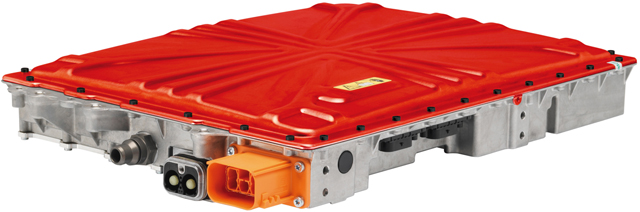
\includegraphics[width = 0.8\textwidth]{figures/brusa_charger.jpg}
	\caption{A svájci BRUSA cég "On-board" töltője} 
	\label{fig:brusa}
\end{figure}

\paragraph{}
Jövőbe tekinthető elképzelés látható \aref{fig:tesla_home} ábrán. A TESLA californiai elktormos autó gáyrtó cég elképzelése a jövő otthonáról, mely megvalósításához rendelkezésre áll a technológia. Az ábrán egy napelemmes cserepekkel burkolt tetejű házat látunk, melynek garázsában található az elektromos autó, illetve a falon a \emph{Powerwall 2.0} nevű akkumulátor csomag, mely az éjszaka folyamán hivatott ellátni a házat elektromossággal. Így tehát megoldódik az otthoni energiaellátás, és a közlekedés problémája is, kevésbé napsütéses időben pedgik akár az uató akkumlátora is szolgálhat tartalékként. A falra szerelhető akkumlátor kapacitása egyébként 14 kWh. Hangaztos elképzelés valóban, de a hálózatról való leszakadásra bizonyosan nem alkalmas, hiszen ha sokáig nem tud megfelelő mennyiségű energiát előállítani a rendszer, bizony kényetelenek leszünk az elektromos hálózatra támaszkodni. 

\begin{figure}[h]
	\centering
	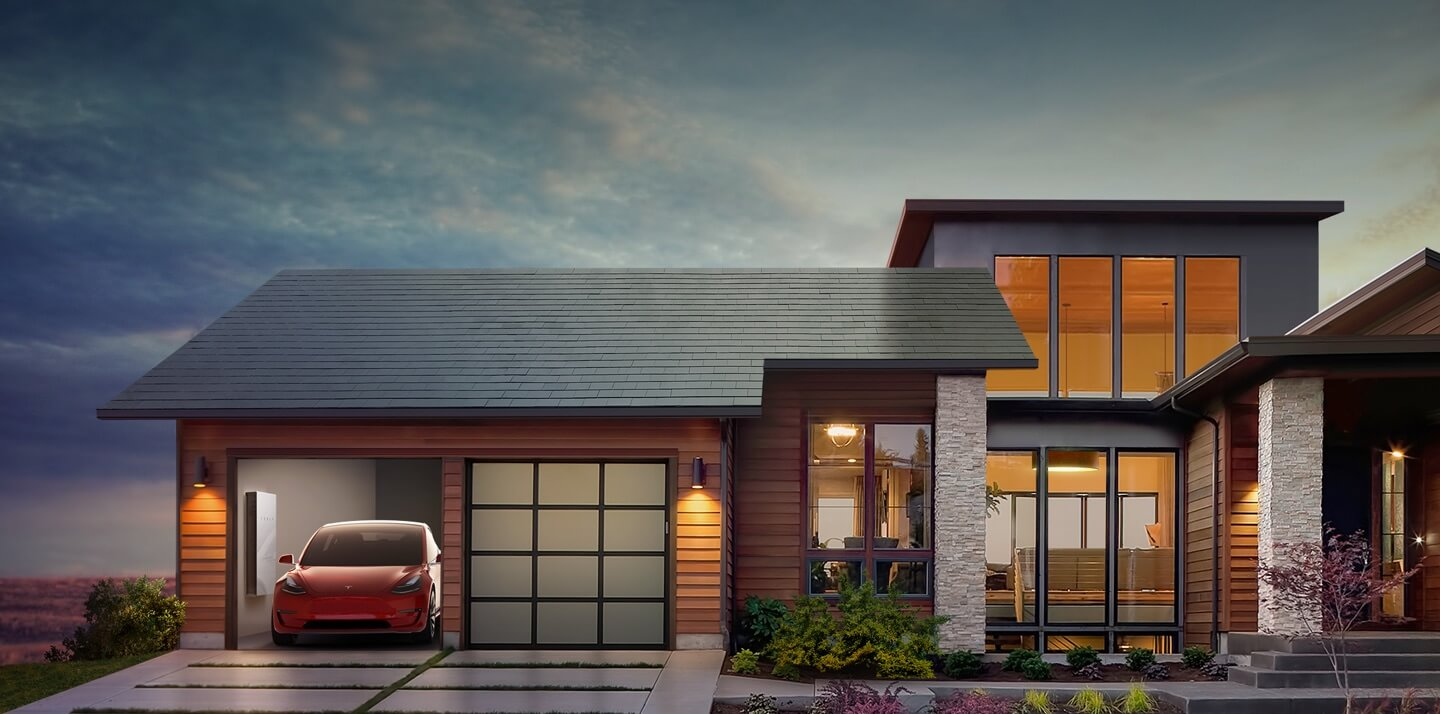
\includegraphics[width = \textwidth]{figures/section-solar.jpg}
	\caption{A TESLA cég elképzelése az integrált otthonról} 
	\label{fig:tesla_home}
\end{figure}



\paragraph{}
A következő probléma az akkumulátorban tárolt energia felhasználása a jármű hajtására. Ehhez nyilvánvalóan szükség van egy motorra, amely többnyire háromfázisú szinkrongép. A fenti elvárások most is adottak, hiszen a ezt az eszközt is folyamatosan magunkkal kell vinni. Az integráció, illetve az egyre nagyobb teljesítménysűrűség elérésének igényét mutatja, hogy ma már több olyan megoldás is létezik, mely egybe integrálja a motort és annak a meghajtó elektornikáját (ami gyakorlatilag egy háromfázisú inverter). \Aref{fig:protean} ábárn látható az angol \emph{PROTEAN} cég kerékagy motorja, mely a fent leírt rendszert valósítja meg. Biztosítani kell számára a DC nagyfeszültséget, a 12 V-os segédüzemű táplálást, valamit CAN buszon a vezérlést. Ez a csomag jelentősen megkönnyíti a járműfejlesztő mérnökök dolgát, hiszen nem kell az autóban még egy dobozt elhelyezniük, menet közben pedig egyszerűen csak nyomaték-alapjelet kell a motoroknak küldeni.

\begin{figure}[h]
	\centering
	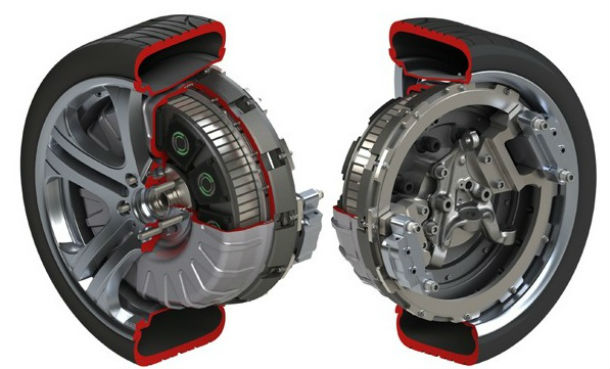
\includegraphics[width = 0.8\textwidth]{figures/protean_motor.jpg}
	\caption{A PROTEAN kerékagymotorja} 
	\label{fig:protean}
\end{figure}

Fenti -- és még sok más egyéb -- húzóágazatok miatt egyre inkább gyorsul a teljesítmény-átalakító eszközök fejlődése, ennélfogva, hogy piacképes terméket lehessen előállítani a fejlesztési időknek is egyre gyorsulnia kell. Ezt támogató eszköz a \emph{Hardware in the Loop} szimulátor. 


\begin{figure}[h]
	\centering
	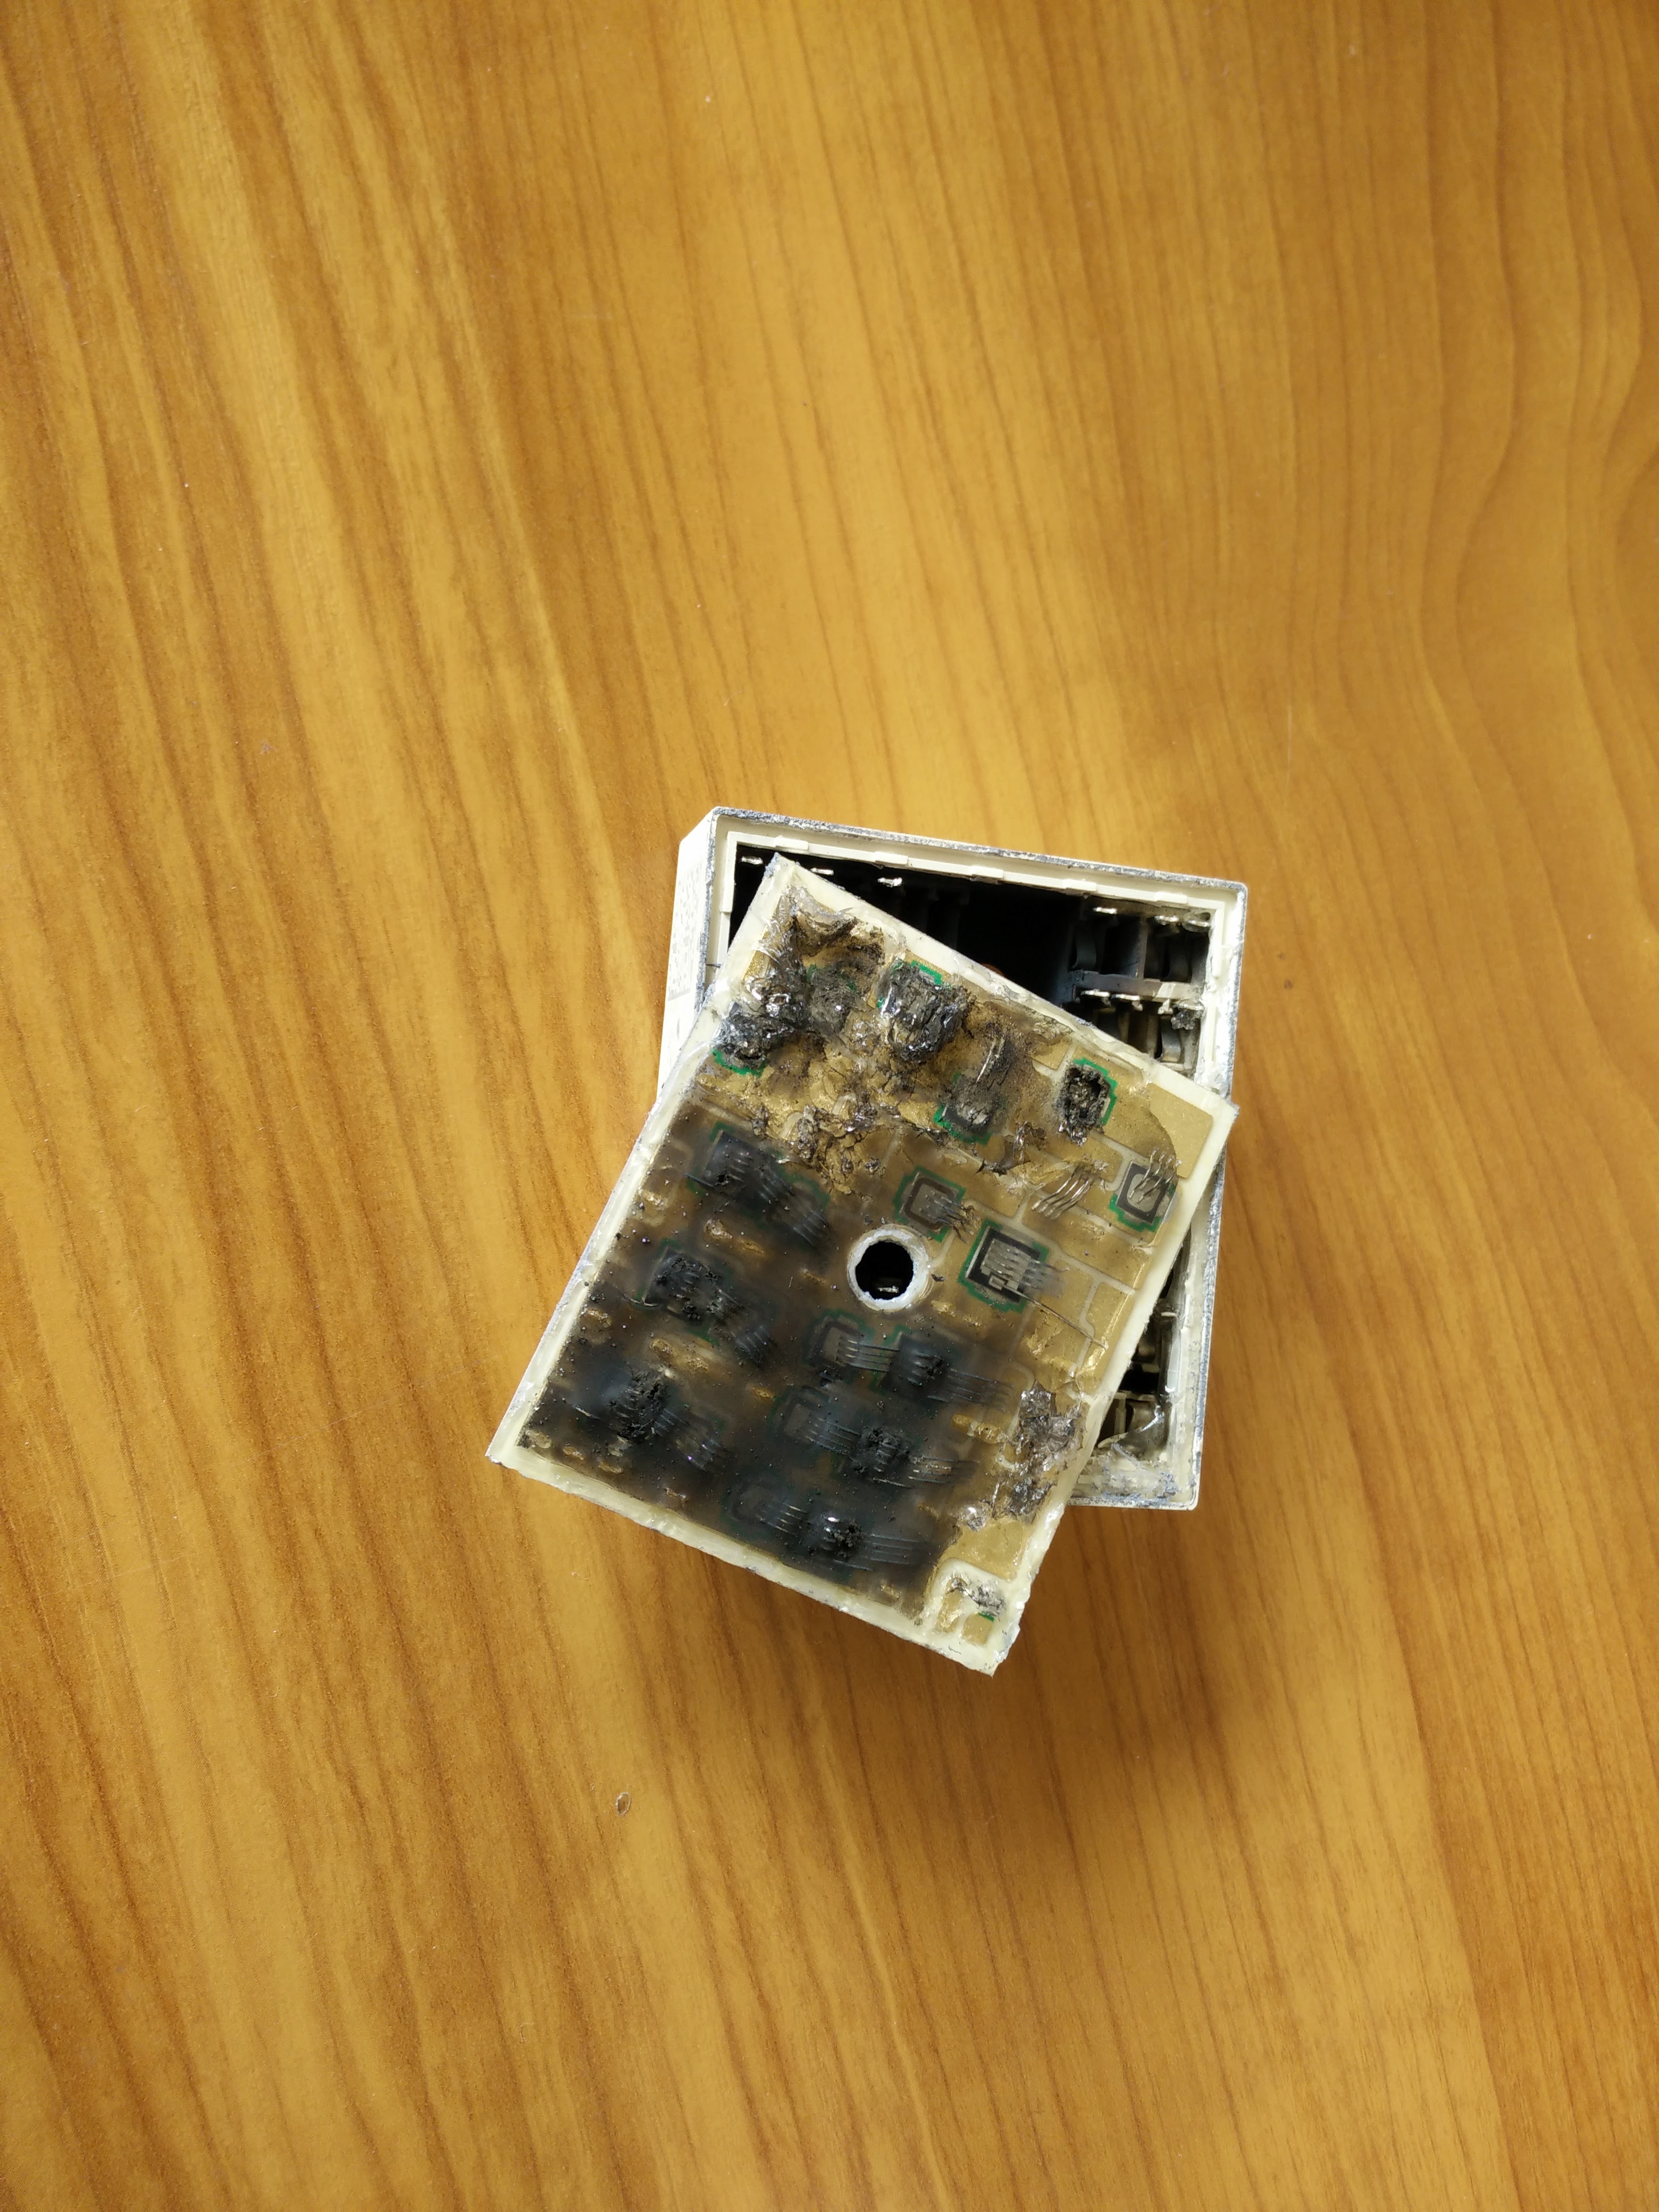
\includegraphics[scale = 0.1]{figures/IMG_20160415_134241.jpg}
	\caption{Felrobbant IGBT modul} 
	\label{fig:blown}
\end{figure}

\paragraph{}
Dolgozatomban végigkísérem egy frekvenciaváltó fejlesztésének folyamatát, különös tekintettel a HIL szimulációra. Megvizsgálom, milyen folyamatok során válik szükségessé, illetve milyen szerepet tölt be az eszköz mind a feljelsztés, mind pedig a tesztelés szakaszában. Maga a teljesítményátalakító tervezése és vezérlése is igen bonylult feladat, ezt egy ipari eszközbe kell becsomagolni, melynek kellően robosztusnak kell lennie, hogy az ennek megfelelő szabványoknak és követelményeknek is megfeleljen. Ezért a kifejtés során igyekszem kitekinteni a fejlesztő csapat sokrétűségére is rugalmasságára is, mely ezt segít megvalósítani.